\section{Pitch rate command system}

Reducing the state space model in Equation~\ref{eq:sslon} by eliminating the velocity and pitch angle states result in the following model.

\begin{equation}
    \begin{aligned}
        A_{red}&=\begin{bmatrix}
            -0.05167 &   0.9792 \\
            -0.6256  & -0.2485
        \end{bmatrix} &
        B_{red}&=\begin{bmatrix}
            -0.0002308 \\
            -0.01541
        \end{bmatrix} \\\\
        C_{red}&=I_2 &
        D_{red}&=0_{2,1}
    \end{aligned}
\end{equation}

Simulating the step response for both models yields similar results. It is clear in the response of the full model that the short period is the dominant eigenmotion during the first few seconds. Since only the initial response of the system in relevant for the CAP and Gibson dropback criterion, it is fine to continue using the reduced model for the rest of the assignment.

\begin{figure}[ht]
    \centering
    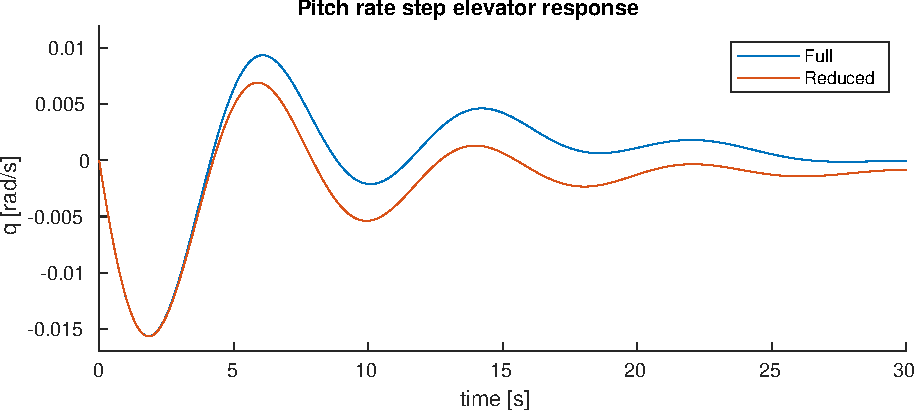
\includegraphics[width=0.6\textwidth]{figures/pc_acre_step.pdf}    
    \caption{Pitch rate elevator step response for both the full and reduced model.}
    \label{fig:pc_acre_step}
\end{figure}

A feedback loop is needed in order to satisfy the short period natural frequency and damping requirements. Figure~\ref{fig:pc_loop1} shows the control loop for solving this problem. The system $G$ is the open loop state space system and $K$ is the to be determined gain matrix.

\begin{figure}[ht]
    \centering
    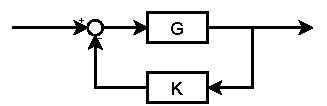
\includegraphics[width=0.4\textwidth]{figures/pc_loop1.pdf}    
    \caption{Feedback loop with gain in the loop.}
    \label{fig:pc_loop1}
\end{figure}

The build-in matlab function \texttt{place(...)} is used to calculate the gain $K_{reduced}$ using pole placement. The resulting gain is shown in Equation~\ref{eq:gaink}. The gain for the longitudinal aircraft model is shown Equation~\ref{eq:gainkac}.

\begin{equation}
    \label{eq:gaink}
    K_{reduced}=\begin{bmatrix}
                    K_{\alpha} & K_q
                \end{bmatrix}
               =\begin{bmatrix}
                    -449.0440 & -151.8325
                \end{bmatrix}
\end{equation}

\begin{equation}
    \label{eq:gainkac}
    K_{a/c}=\begin{bmatrix}
                    0 & K_{\alpha} & 0 & K_q
                \end{bmatrix}
               =\begin{bmatrix}
                    0 & -449.0440 & 0 & -151.8325
                \end{bmatrix}
\end{equation}

The new closed loop system matrix $A$ can then be calculated using Equation~\ref{eq:aclosed} and the rest of the matrices are the same as that of the open loop system. The new closed loop system can be found in Equation~\ref{eq:closedloopsystem}.

\begin{equation}
    \label{eq:aclosed}
    A_{closed} = A_{open}-B_{open}K
\end{equation}


ans =
 
  A = 
                   v       alpha       theta           q
   v        -0.08894       -42.6      -32.17      -14.76
   alpha  -0.0005042     -0.1553  -3.989e-14      0.9442
   theta           0           0           0           1
   q       1.228e-18      -7.544           0      -2.588
 
  B = 
             delta_e
   v        -0.07104
   alpha  -0.0002308
   theta           0
   q        -0.01541
 
  C = 
              v  alpha  theta      q
   v          1      0      0      0
   alpha      0      1      0      0
   theta      0      0      1      0
   q          0      0      0      1
 
  D = 
          delta_e
   v            0
   alpha        0
   theta        0
   q            0
 
Continuous-time state-space model.

\begin{equation}
    \label{eq:closedloopsystem}
    \begin{aligned}
        A_{red}&=\begin{bmatrix}
            -0.08894    &  -42.6   &   -32.17    &  -14.76   \\
            -0.0005042  &  -0.1553 & -3.989e-14  &    0.9442 \\
                     0  &        0 &          0  &         1 \\
             1.228e-18  &   -7.544 &          0  &    -2.588
        \end{bmatrix} &
        B_{red}&=\begin{bmatrix}
              -0.07104 \\
            -0.0002308 \\
                     0 \\
              -0.01541
        \end{bmatrix} \\\\
        C_{red}&=I_4 &
        D_{red}&=0_{4,1}
    \end{aligned}
\end{equation}

                                                                       
Pole              Damping       Frequency      Time Constant  
(rad/seconds)      (seconds)    
                                 
  
-1.37e+00 + 2.37e+00i     5.02e-01       2.74e+00         7.28e-01    
-1.37e+00 - 2.37e+00i     5.02e-01       2.74e+00         7.28e-01 
-4.17e-02 + 1.21e-01i     3.26e-01       1.28e-01         2.40e+01  
-4.17e-02 - 1.21e-01i     3.26e-01       1.28e-01         2.40e+01     

Calculating the damping and natural frequency of the closed loop system shows that the parameters are close to the required $\zeta=0.5$ and $\omega_n=0.03V\approx 2.74$
\begin{table}[h!]
    \centering
    \begin{tabular}{ r | c c c c c }
                     & Poles                           & $\zeta$        & $\omega_n$     \\ \hline \hline
        Short period & $\e{-1.37}{-1} + \e{2.37}{-1}i$ & $\e{5.02}{-1}$ & $\e{2.74}{-1}$ \\  
                     & $\e{-1.37}{-1} - \e{2.37}{-1}i$ & $\e{5.02}{-1}$ & $\e{2.74}{-1}$ \\ \hline
        Phugoid      & $\e{-4.17}{-2} + \e{1.21}{-1}i$ & $\e{3.26}{-1}$ & $\e{1.28}{-1}$ \\   
                     & $\e{-4.17}{-2} - \e{1.21}{-1}i$ & $\e{3.26}{-1}$ & $\e{1.28}{-1}$
    \end{tabular}
    \caption{Longitudinal eigenmotions poles, damping rations, natural frequencies, periods and time to half amplitude.}
\end{table}

If small angle approximations are assumed it is possible to calculate the angle of attack using the following equation.

\begin{equation}
    \alpha = \frac{w}{V}
\end{equation}

Here is $w$ the vertical airspeed component and V the total airspeed. Thus the angle of attack change in case of a vertical gust may be calculated by dividing the gust speed by the free stream velocity. This angle of attack may be passed as an initial condition to a simulation in order to observe the aircraft's behavior during such a gust. For a severe gust with $w=4.572\ [m\ s^{-1}]$ the initial angle of attack in the assigned flight condition is,

\begin{equation}
    \alpha_0=\frac{4.572\ [m\ s^{-1}]}{300\ [ft\ s^{-1}]}=\frac{4.572\ [m\ s^{-1}]}{91.44\ [m\ s^{-1}]} = 0.05\ [rad]
\end{equation}

The simulation results for both the open and closed loop systems using this initial condition and zero inputs is shown in Figure~\ref{fig:pc_vertgust}. As it can be seen the closed loop system quickly dampens the disturbance due the vertical gust, in contrast to the open loop system which continues oscillating significantly longer.

\begin{figure}[ht]
    \centering
    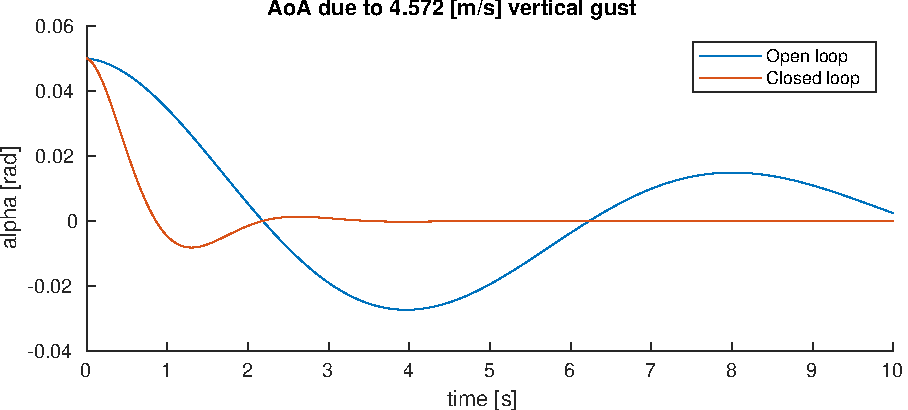
\includegraphics[width=0.6\textwidth]{figures/pc_vertgust.pdf}    
    \caption{Angle of attack during a $w=4.572\ [m\ s^{-1}]$ vertical gust for the open and closed loop systems.}
    \label{fig:pc_vertgust}
\end{figure}

Category B: Those nonterminal Flight Phases that are normally accomplished using
gradual maneuvers and without precision tracking, although accurate
flight-path control may be required. Included in this Category are:


\clearpage
